\documentclass[a4paper,utf8]{article}
\usepackage[heading,fancyhdr]{ctex}
\usepackage{amsmath,amssymb,geometry,lastpage,ulem}
\usepackage{array,tabularx,tabulary,mhchem,xspace}
\usepackage{floatrow,subfig,multirow,bigstrut}
\usepackage{siunitx,booktabs,longtable,graphicx,xfrac,nameref}
\lineskiplimit=1pt
\lineskip=3pt
\geometry{
    top=25.4mm, 
    left=25mm, 
    right=25mm, 
    bottom=25mm,
    headsep=5.9mm,
}
\ctexset{
    section = {format+=\raggedright}
}
\newcommand{\fgref}[1]{图~\ref{#1}\xspace}
\newcommand{\seqref}[1]{式~(\ref{#1})}
\newcommand{\expinfo}[7][无]{
    {\zihao{-3}\bfseries\songti
    实验名称:\uline{\hfill\mbox{#2}\hfill} \\[2.9mm]
    学\quad 号:\uline{\makebox[25mm]{#3}}\hfill
    姓\quad 名:\uline{\makebox[25mm]{#4}}\hfill
    班\quad 级:\uline{\makebox[25mm]{#5}} \\[2.9mm]
    合作者:\uline{\makebox[25mm]{#1}} \hfill
    桌\quad 号:\uline{\makebox[25mm]{#6}}\hfill\makebox[25mm+4em]{}\\[2.9mm]
    实验日期:\uline{\makebox[30mm]{#7}}\hfill\mbox{} \\[58.7mm]
    }
}
\newcommand{\pointingbox}{
    {\zihao{4}\bfseries\songti%
    实验考核\\[3mm]
    \extrarowheight=3mm
    \begin{tabularx}{150mm}{|X|X|X|X|X|}\hline
        \hfil 项目 \hfil  & \hfil 实验预习 \hfil & \hfil 实验过程 \hfil & \hfil 分析与讨论 \hfil & \hfil 总评 \hfil \\[3mm] \hline
        \hfil 评价 \hfil &  &  &  &  \\[3mm] \hline
    \end{tabularx}
    }
}
\newcommand{\derivative}[2]{\frac{\mathrm{d} #1}{\mathrm{d} #2}}
\newcommand{\thinking}[2]{\textbf{#1}\\
答:\begin{minipage}[t]{0.85\textwidth}
    #2
\end{minipage}}
\pagestyle{fancy}
\fancyhf{} \fancyhead[C]{电路基础实验} \fancyfoot[C]{\thepage~/~\pageref{LastPage}}
\newcounter{Rownumber}
\newcommand*{\Rown}{\stepcounter{Rownumber}\theRownumber}
\newcommand*{\resetRown}{\setcounter{Rownumber}{0}}
\newcommand{\qrange}[3]{\qtyrange[range-phrase = \text{$\sim$},range-units =single]{#1}{#2}{#3}}
\floatsetup[table]{capposition=top}
\newcolumntype{C}{>{\hfil}X<{\hfil}}
\renewcommand{\Nameref}[1]{\textbf{\ref{#1}~\nameref{#1}}} %导入导言
\usepackage{picinpar}
\newcommand*{\Usa}{$V_1$}
\newcommand*{\Usb}{$V_2$}
\ctikzset{
    resistors/scale=0.7,
    diodes/scale=0.6}
\begin{document}
\begin{center}
    {\mbox{}\\[7em]\zihao{2}\bfseries\songti%
    电路基础实验报告}\\[34mm]
    \expinfo[王慷]{电压源和电流源的转换}{22301056}{王俊杰}{22 材物}{27}{2024.5.14}
\end{center}
\newpage
\section{实验目的}
\begin{enumerate}
    \item 掌握电源外特性的测试方法。
    \item 验证电压源与电流源等效变换的条件。
\end{enumerate}

\section{实验原理}%简单描述,含必要的公式和附图;
一个直流电压源在一定的电流范围内,具有很小的内阻,故在实用中,常将它视为一个理想的电压源,即其输出电压不随负载改变而变化。其外特性曲线,即伏安特性曲线 U=f(I)是一条平行于 I 轴的直线。一个电流源在一定的电压范围内,具有很大的内阻,在实用中,可视为一个理想的电流源,即其输出电流不随负载改变而变化。\par
理想电压源实际上是不存在的,实际电压源总具有一定的能量损失,这种实际电压源可以用理想电压源与电阻的串联组合来作为模型。其端口的电压与电流的关系为:
\begin{equation}
    U = U_\text{s} - I R_\text{s}
\end{equation}
式中电阻 $R_\text{s}$ 为实际电压源的内阻,上式的关系曲线如图 3-2 所示。显然实际电压源的内阻越小,其特性越接近理想电压源。同样,一个实际电流源可用电流源和一个大电阻的并联组合来作为模型。\par
一个实际的电源,就其外部特性而言,既可以看成是一个电压源,又可以看成是一个电流源。若视为电压源,则可用一个理想的电压源 $U_\text{s}$ 与一个电阻 $R_\text{o}$ 相串联的组合来表示;若视为电流源,则可用一个理想电流源 $I_\text{s}$ 与一电导 $R_\text{o}$ 相并联的组合来表示。如果这两种电源能向同样大小的负载供出同样大小的电流和端电压,则称这两个电源是等效的,即具有相同的外特性。一个电压源与一个电流源等效变换的条件为:$I_\text{s}=U_\text{s}/R_\text{o}$,或 $U_\text{s}=I_\text{s} R_\text{o}$
\section{实验仪表}
    RIGOL DM3058 万用表、RIGOL DP832 直流稳压电源、电路分析实验箱、导线若干。
\section{实验内容及实验数据}
\subsection{测定电压源的外特性}
\subsubsection{测定理想电压源的外特性}
调节直流稳压电源输出电压 $U=\SI{6}{\V}$,使 $R_\text{L}$ 分别等于 \SI{600}{\ohm}、\SI{500}{\ohm}、\SI{400}{\ohm}、\SI{300}{\ohm}、\SI{200}{\ohm}、\SI{100}{\ohm},将相应的电压、电流数值记入表 \ref{tab:1} 中。
\begin{table}[!ht]
    \centering\begin{tabular}{c c c c c c c c}\toprule
        $R_L (\unit{\ohm})$ & 开路 & 600 & 500 & 400 & 300 & 200 & 100 \\ \midrule
        $U (\unit{\V})$ & 6 & 5.984 & 5.950 & 5.946 & 5.950 & 5.967 & 5.947 \\
        $I (\unit{\mA})$ & 0 & 10.03 & 11.67 & 14.69 & 19.91 & 29.15 & 58.09 \\ \bottomrule
    \end{tabular}\caption{理想电压源测量数据}\label{tab:1}
\end{table}
\subsubsection{测定实际电压源的外特性}
首先选取一个 \SI{51}{\ohm} 的电阻,作为电压源的内阻与电压源串联组成一个实际电压源模型,其中负载电阻仍然取 \SI{600}{\ohm}、\SI{500}{\ohm}、\SI{400}{\ohm}、\SI{300}{\ohm}、\SI{200}{\ohm}、\SI{100}{\ohm},将相应的电压、电流数值记入表 \ref{tab:2} 中。
\begin{table}[!ht]
    \centering\begin{tabular}{c c c c c c c c}\toprule
        $R_L (\unit{\ohm})$ & 开路 & 600 & 500 & 400 & 300 & 200 & 100 \\ \midrule
        $U (\unit{\V})$ & 6 & 5.517 & 5.431 & 5.309 & 5.117 & 4.774 & 3.973 \\
        $I (\unit{\mA})$ & 0 & 9.254 & 10.92 & 13.33 & 17.12 & 23.87 & 39.63 \\ \bottomrule
    \end{tabular}\caption{实际电压源测量数据}\label{tab:2}
\end{table}
\subsection{测定电流源的外特性}
\subsubsection{测定理想电流源的外特性}
设置稳压电源为恒流源模式,电流为 \SI{20}{\mA},使负载 $R_\text{L}$ 分别为 \SI{600}{\ohm}、\SI{500}{\ohm}、\SI{400}{\ohm}、\SI{300}{\ohm}、\SI{200}{\ohm}、\SI{100}{\ohm}、\SI{0}{\ohm},将相应的电压、电流数值记入表 \ref{tab:3} 中。
\begin{table}[!ht]
    \centering\begin{tabular}{c c c c c c c c}\toprule
        $R_L (\unit{\ohm})$ & 600 & 500 & 400 & 300 & 200 & 100 & 0 \\ \midrule
        $U (\unit{\V})$ & 20.15 & 19.83 & 19.83 & 19.75 & 19.72 & 19.73 & 19.74 \\
        $I (\unit{\mA})$ & 11.98 & 9.85 & 7.88 & 5.89 & 3.88 & 1.95 & 0 \\ \bottomrule
    \end{tabular}\caption{理想电流源测量数据}\label{tab:3}
\end{table}
\subsubsection{测定实际电流源的外特性}
$R_\text{s}=\SI{1}{\kilo\ohm}$,设置稳压电源为恒流源模式,电流为 \SI{20}{\mA},使负载 $R_\text{L}$ 分别为 \SI{600}{\ohm}、\SI{500}{\ohm}、\SI{400}{\ohm}、\SI{300}{\ohm}、\SI{200}{\ohm}、\SI{100}{\ohm}、\SI{0}{\ohm},将相应的电压、电流数值记入表 \ref{tab:4} 中。
\begin{table}[!ht]
    \centering\begin{tabular}{c c c c c c c c}\toprule
        $R_L (\unit{\ohm})$ & 600 & 500 & 400 & 300 & 200 & 100 & 0 \\ \midrule
        $U (\unit{\V})$ & 20.15 & 19.83 & 19.83 & 19.75 & 19.72 & 19.73 & 19.74 \\
        $I (\unit{\mA})$ & 11.98 & 9.85 & 7.88 & 5.89 & 3.88 & 1.95 & 0 \\ \bottomrule
    \end{tabular}\caption{理想电流源测量数据}\label{tab:4}
\end{table}
\subsection{测定电源等效变换的条件}
\begin{table}[!ht]
    \centering\begin{tabular}{|c|>{\hfil}m{5em}|}\hline
        电流源供电时 $U (\unit{\V})$ & 1.92  \\\hline
        电流源供电时 $I (\unit{\mA})$ & 9.58 \\\hline
        保持读数不变时所需的电压源 $U_\text{s} (\unit{\V})$ & 2.452 \\ \hline
    \end{tabular}\caption{等效变换条件测量}
\end{table}
\section{实验结果与分析}
\subsection{电源特性曲线}
将电源外特性测量结果绘制为特性曲线,如图 \ref{fig:curve} 所示。可以看出实际的电源的特性曲线接近一条直线且斜率为负数。
\begin{figure}[!ht]
    \caption{电源特性曲线}\label{fig:curve}
    \subfloat[理想电压源的特性曲线]{\includegraphics[width=0.47\textwidth]{1.pdf}}
    \subfloat[实际电压源的特性曲线]{\includegraphics[width=0.47\textwidth]{2.pdf}}\\
    \subfloat[理想电流源的特性曲线]{\includegraphics[width=0.47\textwidth]{3.pdf}}
    \subfloat[实际电流源的特性曲线]{\includegraphics[width=0.47\textwidth]{4.pdf}}
\end{figure}
\subsection{电源等效变换的条件}
根据电源等效变换的公式可计算出
\begin{equation}
    U^{'}_\text{s}=I_\text{s} R_\text{s} = \SI{50}{\mA} \times \SI{51}{\ohm} = \SI{2.55}{\V}
\end{equation}\par
实际测量的相对误差
\begin{equation}
    E=\frac{\left|U_\text{s}-U^{'}_\text{s}\right|}{U^{'}_\text{s}}\times 100 \% =\frac{\left|2.55-2.452\right|}{2.55}\approx 3.84\%
\end{equation}
\section{实验心得}
这次实验设计了几个电路测量电源的外特性,并且验证了电源等效变换的条件。在实际操作中,观察到了由于仪器误差和连接线电阻带来的微小偏差,但总体上实验结果符合理论预期。这些实验加深了我对实际电源的理解。
\section{原始数据}
\begin{center}
    \framebox{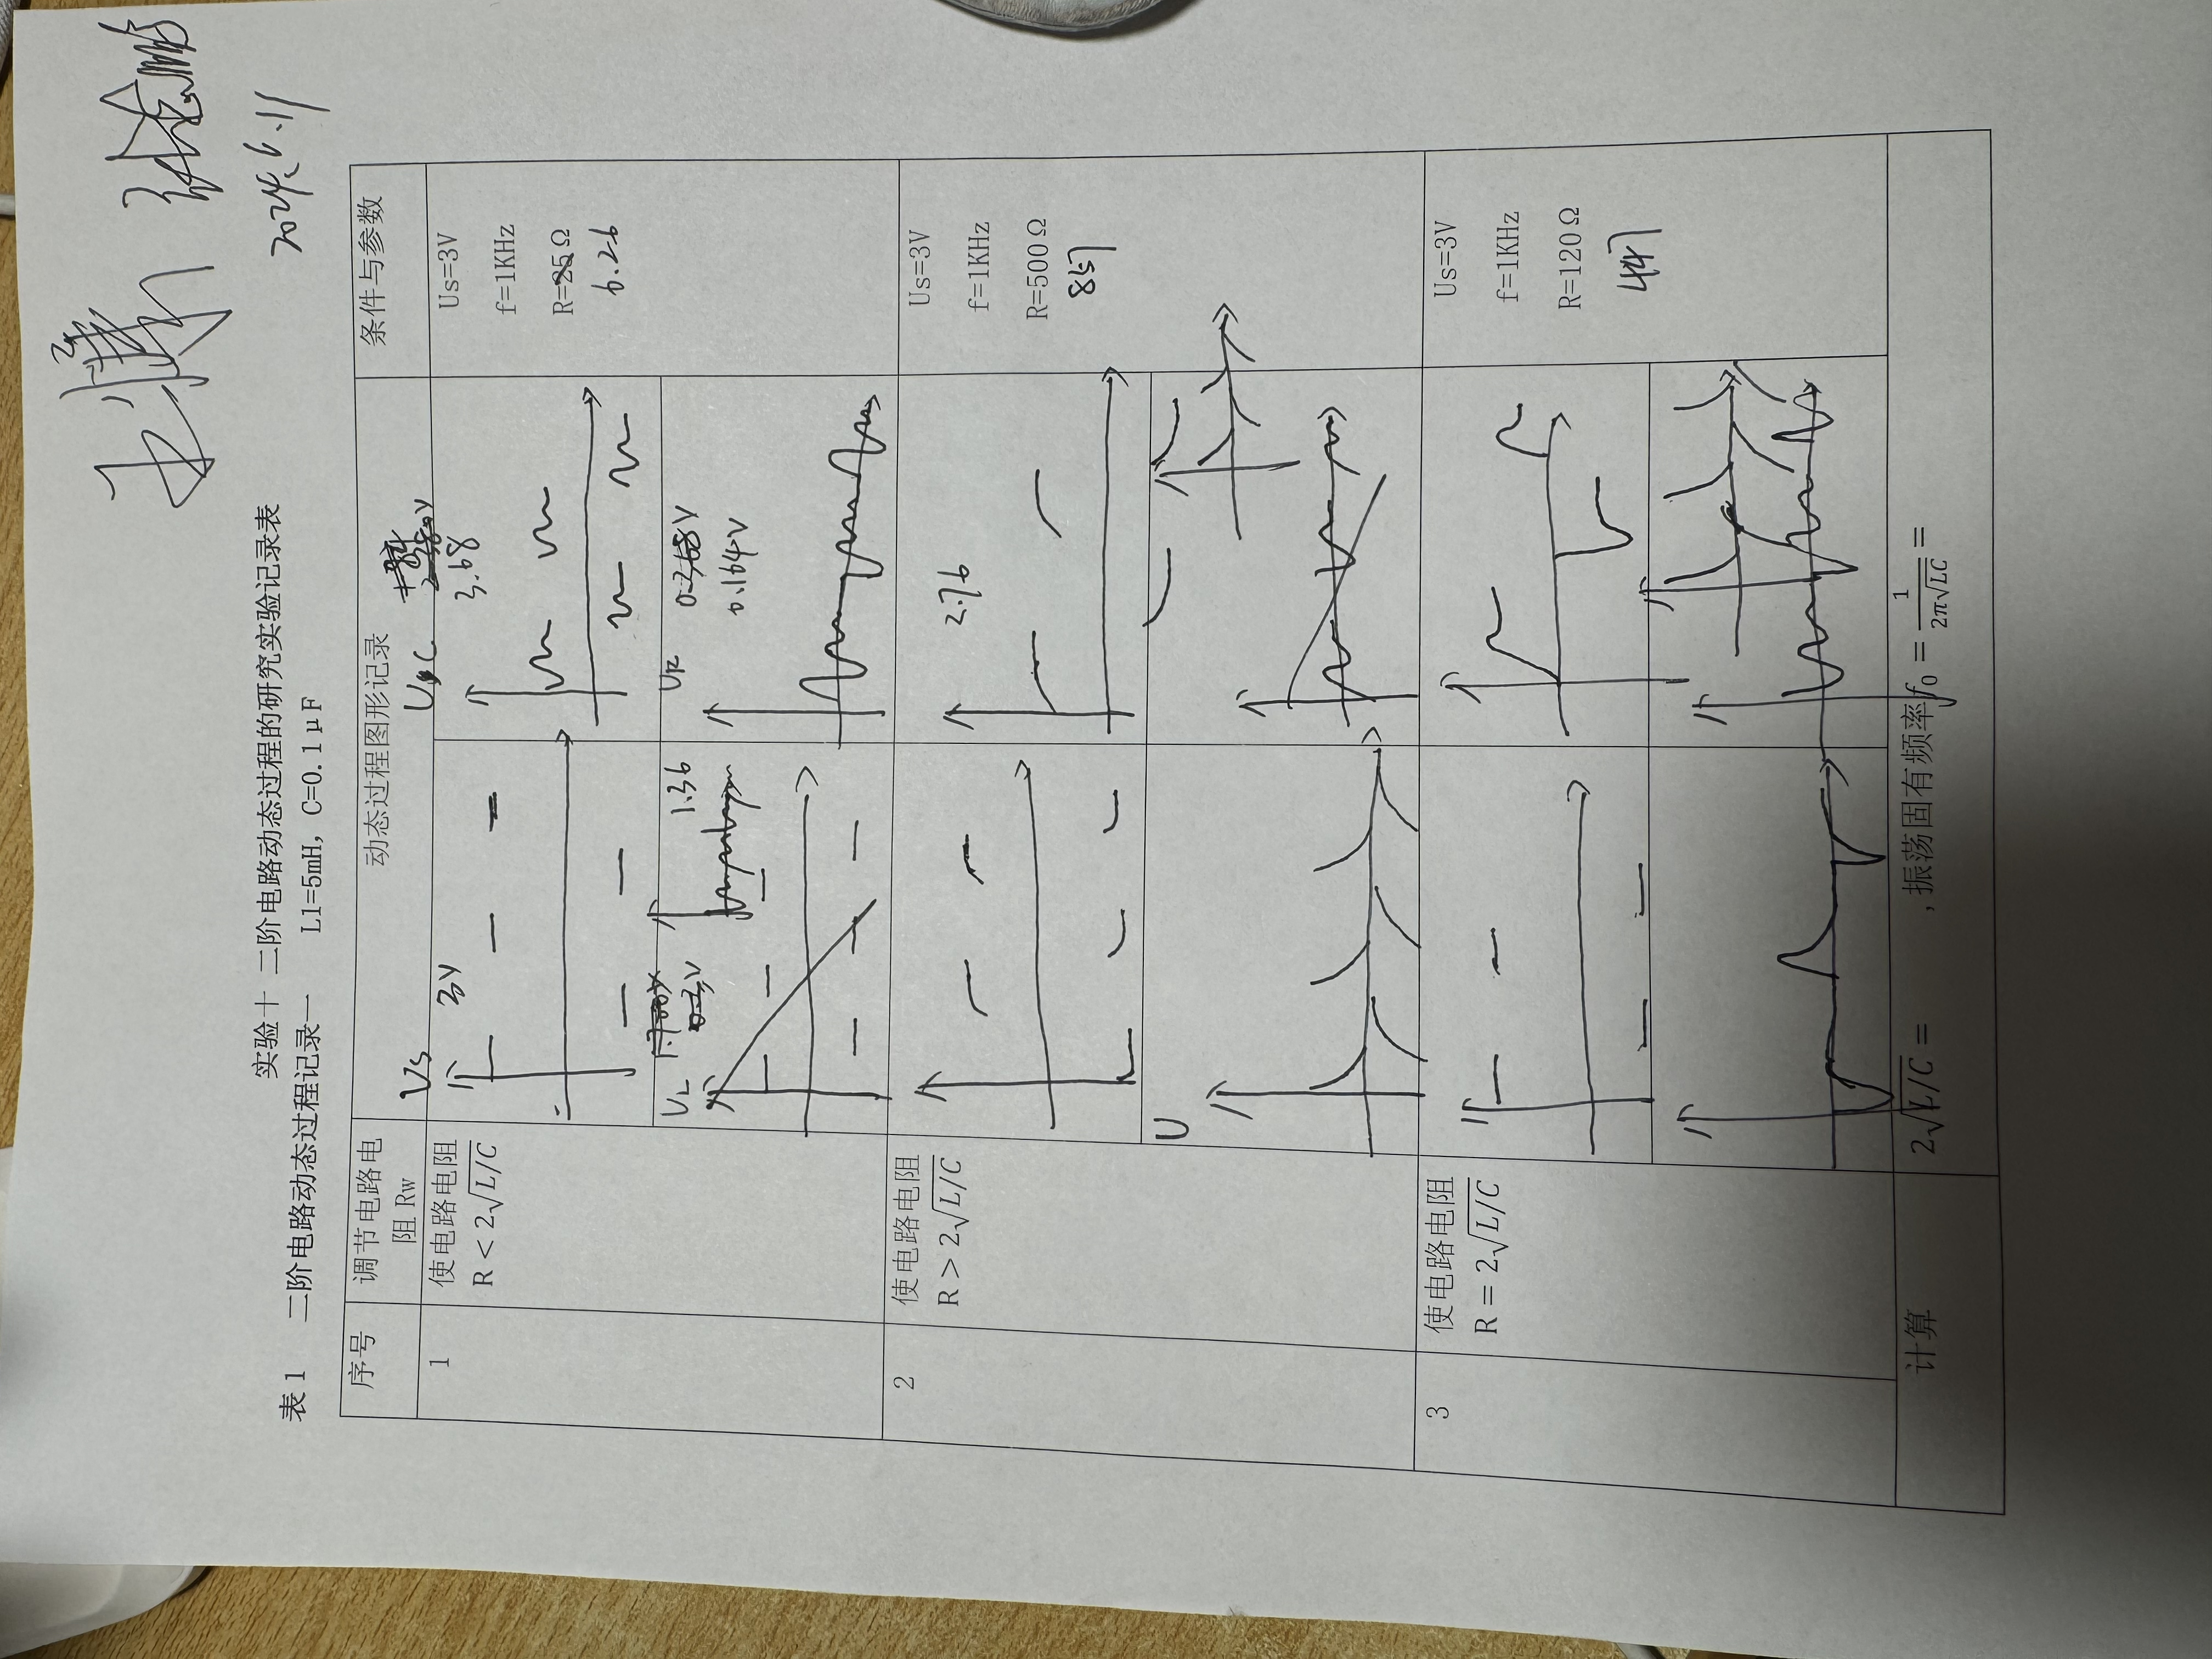
\includegraphics[width=0.8\textwidth]{rawdata.jpg}}
\end{center}

\end{document}